\chapter{Marco Metodológico}

\section{Arquitectura del sistema híbrido}

El sistema propuesto se basa en una arquitectura híbrida que combina modelado mecanístico y aprendizaje automático para superar las limitaciones de los enfoques puramente empíricos o puramente físicos. Esta arquitectura opera en tres niveles funcionales:

\section{Justificación de la Arquitectura Híbrida Inteligente}

El sistema se fundamenta en una arquitectura de procesamiento en tres etapas, diseñada para extraer información de valor a partir de sensores de bajo costo, sin requerir una infraestructura de control industrial compleja:

\textbf{1. Estimación de variables latentes (Sensor Virtual):} El modelo mecanístico (EDO), alimentado con las series de tiempo de los sensores IoT (temperatura, \ce{CO2}, humedad) durante las ventanas de medición, permite inferir variables biológicas no medibles directamente, como la tasa metabólica instantánea. Esta funcionalidad, conocida como \textit{soft-sensor}, busca convertir el dato físico crudo (ppm de gas) en una representación dinámica del estado de actividad larval \parencite{liuOptimizingDataPipelines2023}.

\textbf{2. Corrección dinámica mediante aprendizaje automático:} Reconociendo que los modelos teóricos son sensibles a la heterogeneidad del residuo (variabilidad no modelada), el sistema implementa una corrección aditiva del error. Un algoritmo de aprendizaje ligero (ej. Regresión o Random Forest) estima el \textit{residuo} o discrepancia entre la curva teórica del EDO y la medición real del sensor. Este valor se suma a la predicción base para ajustar el resultado final sin alterar los parámetros fisiológicos del modelo. Este enfoque híbrido mejora la precisión local manteniendo la interpretabilidad biológica del modelo global.

\textbf{3. Soporte preventivo a la decisión (Alerta Temprana):} Mediante la proyección a corto plazo (15–30 minutos) de la tendencia de \ce{CO2} y su correlación con la humedad, el sistema busca identificar patrones de estancamiento o saturación que preceden a la formación de focos anaerobios (generadores de \ce{CH4}). Esta capacidad de anticipación habilita una gestión preventiva: el sistema puede generar alertas de \textit{Riesgo de Anaerobiosis} para sugerir intervenciones manuales (como el volteo), optimizando el desempeño ambiental antes de que se consoliden emisiones significativas.

\section{Ubicación y Contexto Experimental}

El componente experimental se desarrollará en la sede Palmira de la Universidad Nacional de Colombia, ver Figura \ref{fig:localizacion}). La zona se caracteriza por corresponder a un ecosistema de bosque tropical seco, con una temperatura media anual de $24^\circ C$, condiciones que favorecen el desarrollo natural de \textit{Hermetia illucens}. El montaje se realizará en condiciones de laboratorio controlado (mesocosmos) para garantizar la reproducibilidad de los datos de calibración.

\begin{figure}[h]
    \centering
    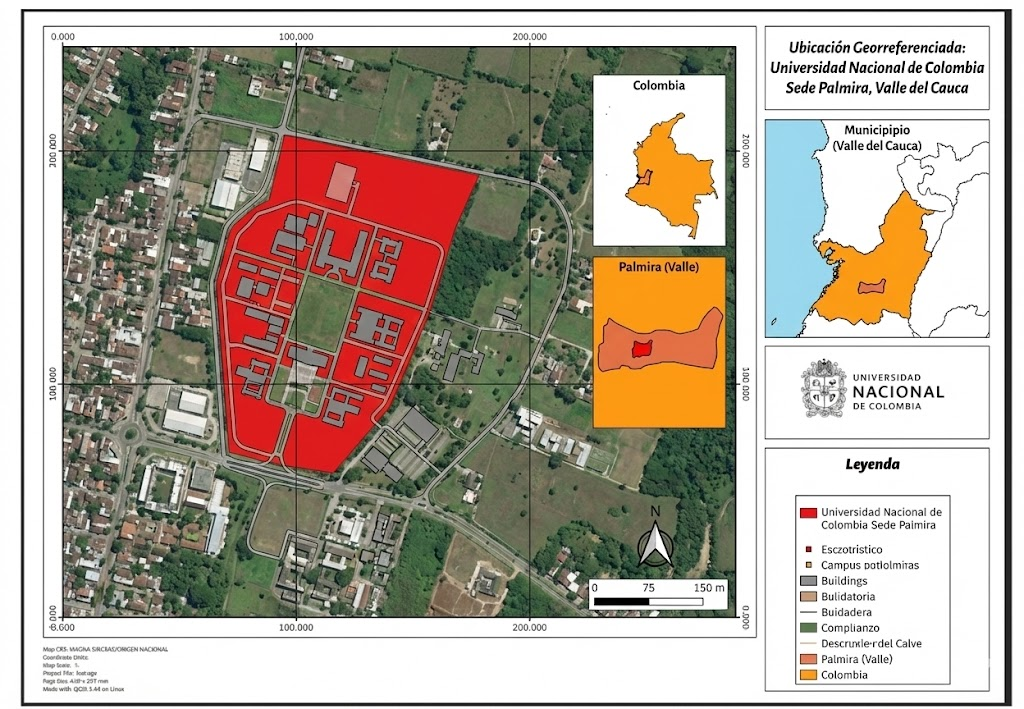
\includegraphics[width=0.8\textwidth]{00Figuras/localizacion.jpg} % Asegúrate de que la ruta sea correcta
    \caption{Ubicación del proyecto en Palmira, Valle del Cauca, Colombia.}
    \label{fig:localizacion}
\end{figure}

\section{Enfoque y Tipo de Investigación}

Este estudio se enmarca dentro de una investigación aplicada, experimental, tecnocientífica e interdisciplinaria, orientada al desarrollo y validación de un sistema híbrido para la caracterización dinámica de emisiones de gases de efecto invernadero (GEI).

El enfoque es cuantitativo, fundamentado en la recolección sistemática de series de tiempo mediante sensores IoT, el modelado determinista (EDO) y el análisis estadístico predictivo (Machine Learning). La metodología se estructura en cuatro fases secuenciales e integradas que van desde la instrumentación física hasta la validación de la utilidad ambiental del sistema.

\section{Diseño Experimental y Desarrollo (Materiales y Métodos)}

\subsection{Fase I: Diseño e Implementación del Sistema IoT y Aseguramiento de Datos}

El objetivo de esta fase es garantizar la calidad del dato de entrada. Dada la naturaleza agresiva del entorno de bioconversión (alta humedad relativa $>80\%$), se implementarán protocolos de robustez instrumental.

\textbf{Actividades Clave:}
\begin{itemize}
    \item \textbf{Implementación de Hardware:} Diseño de un nodo de sensores basado en microcontroladores (tipo ESP32), integrando sensores NDIR para \ce{CO2} y semiconductores/electroquímicos para \ce{CH4}.
    \item \textbf{Protocolos de Calibración:} Ejecución de curvas de calibración frente a concentraciones patrón y desarrollo de algoritmos de \textbf{compensación cruzada} para corregir la deriva del sensor causada por las fluctuaciones de temperatura y humedad inherentes al proceso exotérmico.
    \item \textbf{Captura de Datos:} Despliegue de la red IoT para la recolección de datos en ciclos de bioconversión (14-20 días), generando el \textit{dataset} experimental necesario para el entrenamiento de los modelos.
\end{itemize}

\subsection{Fase II: Parametrización del Modelo Mecanístico (Línea Base)}

Se formulará un modelo matemático basado en Ecuaciones Diferenciales Ordinarias (EDO) bajo el marco del \textit{Dynamic Energy Budget} (DEB) simplificado. Este modelo tendrá como función exclusiva describir la tendencia ideal aerobia del proceso.

\textbf{Enfoque de Modelado:}
\begin{itemize}
    \item El modelo EDO describirá el crecimiento larval y la producción respiratoria de \ce{CO2} asumiendo condiciones óptimas de operación.
    \item Se asume que el \ce{CH4} responde a anomalías estocásticas (focos anaerobios) que escapan a la cinética determinista estándar, por lo que su modelado se delega a la fase híbrida.
    \item \textbf{Resultado:} Una curva teórica de referencia ($Y_{modelo}$) que servirá de línea base para detectar desviaciones operativas.
\end{itemize}

\subsection{Fase III: Desarrollo del Sistema Híbrido (Detección y Corrección)}

En esta fase se integra la Inteligencia Artificial para cerrar la brecha entre la teoría (Fase II) y la realidad observada (Fase I).

\textbf{Estrategia Híbrida:}
\begin{itemize}
    \item \textbf{Cálculo del Residual:} Se calculará la diferencia instantánea entre el dato del sensor y la predicción del modelo EDO ($\epsilon = Y_{sensor} - Y_{modelo}$).
    \item \textbf{Entrenamiento de Algoritmos:} Se entrenarán modelos de regresión (ej. Random Forest o Redes Neuronales ligeras) para predecir este error residual en función de las variables ambientales, ajustando así la estimación final.
    \item \textbf{Detección de Anomalías (\ce{CH4}):} Se implementará un clasificador para identificar patrones de "firma espectral" (ej. estancamiento de \ce{CO2} acoplado a alta humedad) que correlacionen con picos de \ce{CH4}, permitiendo una detección indirecta o "soft-sensing" de la anaerobiosis.
\end{itemize}

\subsection{Fase IV: Validación Ambiental y Soporte a la Decisión}

La fase final busca validar la utilidad de la información generada para la gestión operativa y el reporte ambiental.

\textbf{Validación:}
\begin{itemize}
    \item \textbf{Comparativa de Escenarios:} Se analizará el desempeño del sistema procesando datos de sustratos contrastantes para verificar su sensibilidad en la discriminación de perfiles de emisión.
    \item \textbf{Validación del Reporte:} Se cuantificarán las emisiones totales del ciclo para obtener un indicador de desempeño ambiental. Este resultado se comparará con la literatura para confirmar que la medición en sitio mejora la calidad del reporte.\end{itemize}

\section{Arquitectura Tecnológica del Sistema}

El sistema sigue una arquitectura modular de tres capas, diseñada bajo el paradigma IoT para garantizar la integridad, disponibilidad y trazabilidad del dato científico (Ver Figura \ref{fig:arquitectura}):

\subsection{Capa de Percepción (Edge Computing)} Compuesta por el nodo sensor (Hardware basado en ESP32). Su función principal es la digitalización de variables físicas. Para garantizar la robustez del dato experimental, esta capa implementa: \begin{itemize} \item Adquisición y Filtrado: Lectura de sensores y aplicación de filtros digitales (media móvil) para atenuar el ruido eléctrico. \item Resiliencia: Almacenamiento temporal en memoria local (SD/Flash) para evitar pérdida de datos ante fallos de conectividad (buffer circular). \item Telemetría: Transmisión asíncrona de la trama de datos mediante protocolo ligero MQTT hacia el servidor de procesamiento. \end{itemize}

\subsection{Capa de Procesamiento (Core/Cloud)} Módulo de software centralizado donde reside la lógica científica del sistema. \begin{itemize} \item Gestor de Datos (Ingesta): Recibe la telemetría, realiza una validación de rangos (sanitización de datos) y la almacena en una base de datos relacional para garantizar la persistencia histórica. \item Motor Híbrido de Estimación: Ejecuta secuencialmente el modelo matemático: primero resuelve la cinética base (EDO) y posteriormente invoca el algoritmo de aprendizaje automático para corregir el error residual, generando la "Variable Estimada"\ final. \end{itemize}

\subsection{Capa de Aplicación (Interfaz de Decisión)} Interfaz de visualización orientada al usuario final y al soporte de decisiones operativas. Sus funcionalidades clave incluyen: \begin{itemize} \item Monitorización Dinámica: Visualización de las curvas de tendencia (Real vs. Estimada) en tiempo real. \item Auditoría Ambiental: Módulo de descarga de reportes consolidados del ciclo para procesos de MRV. \item Gestión de Alertas: Semáforo de riesgo que notifica visualmente la detección de patrones compatibles con anaerobiosis incipiente. \end{itemize}

\begin{figure}[h!] \centering \includegraphics[width=1.0\textwidth]{00Figuras/DG_FLUJO_GENERAL.png} \caption{Diagrama de la arquitectura funcional del sistema de monitoreo y predicción híbrido, detallando el flujo de datos desde la percepción física hasta la toma de decisiones.} \label{fig:arquitectura} \end{figure}

\section{Criterios de Validación y Métricas de Éxito}

Para evaluar el cumplimiento de los objetivos, se establecen los siguientes umbrales de desempeño:

\begin{itemize}
    \item \textbf{Robustez Instrumental:} Se aceptará una correlación de Pearson ($R > 0.85$) entre la señal del sensor y la tendencia esperada, con un error porcentual medio (MAPE) $< 15\%$, considerando las limitaciones técnicas de los sensores \textit{low-cost} en ambientes de saturación hídrica.
    
    \item \textbf{Mejora Híbrida:} El sistema híbrido (EDO + IA) se considerará exitoso si logra reducir el error de predicción (RMSE) en al menos un 20\% en comparación con el uso del modelo mecanístico (EDO) por sí solo.
    
    \item \textbf{Sensibilidad a Anomalías:} Se validará la capacidad del sistema para identificar correctamente los eventos de pico de metano (Clasificación Binaria: Presencia/Ausencia de Anaerobiosis) con una métrica de Sensibilidad (\textit{Recall}) $> 80\%$, priorizando la minimización de falsos negativos.
    
    \item \textbf{Utilidad MRV:} El sistema deberá ser capaz de generar automáticamente un reporte de emisiones acumuladas al final del ciclo, coherente con los balances de masa teóricos calculados por métodos de referencia.
\end{itemize}

\section{Alineación de Objetivos y Estrategia Experimental}
A modo de síntesis, la Tabla~\ref{tab:resumen_metodologia} presenta la matriz de coherencia que articula los objetivos específicos con sus respectivas fases de ejecución y criterios de validación. Esta estructura evidencia que el diseño metodológico no opera como un conjunto de técnicas aisladas, sino como un sistema integrado en el que la calidad de las mediciones instrumentales (Fase I), la solidez del modelo mecanístico (Fase II) y la capacidad de corrección basada en datos (Fase III) se articulan de manera coherente. Este enfoque permite que cada fase contribuya de forma directa y cuantificable al desarrollo de una herramienta de gestión ambiental (Fase IV), asegurando la trazabilidad científica desde la captura de la señal hasta la toma de decisiones operativas.

\begin{table}[h]
\centering
\caption{Matriz de Coherencia Metodológica}
\label{tab:resumen_metodologia}
\begin{tabular}{|p{3cm}|p{4cm}|p{4cm}|p{3cm}|}
\hline
\textbf{Objetivo Específico} & \textbf{Método / Fase} & \textbf{Entregable Clave} & \textbf{Criterio de Éxito} \\ \hline
1. Hardware IoT & Fase I: Diseño e Implementación & Dataset experimental (14 días) & $R > 0.85$ (coeficiente de Pearson vs. referencia) \\ \hline
2. Modelo EDO & Fase II: Parametrización & Simulación de referencia de \ce{CO2} & MAPE $< 15\%$ en ventana de 30 min \\ \hline
3. Sistema Híbrido & Fase III: Desarrollo Algorítmico & Motor de corrección de error & Reducción del RMSE $\geq 20\%$ frente al modelo EDO \\ \hline
4. Validación & Fase IV: Evaluación Ambiental & Reporte MRV y sistema de alertas & Recall $> 80\%$ en detección de eventos de estrés metabólico \\ \hline
\end{tabular}
\end{table}

\section{Análisis Crítico: Limitaciones, Riesgos y Desafíos de Implementación}

Si bien la integración de tecnologías digitales promete optimizar la bioconversión, este estudio adopta una postura \textit{tecno-realista}, reconociendo que la digitalización no es neutral ni está exenta de externalidades. En respuesta a la necesidad de un análisis riguroso sobre la viabilidad técnica y socioambiental, a continuación se detallan las tensiones éticas, ambientales, epistémicas y operativas inherentes a la propuesta, junto con las estrategias de mitigación integradas en su diseño.

\subsection{Tensión socioecológica: impacto de la materialidad digital}
Existe una tensión entre la sostenibilidad del proceso biológico (bioconversión) y la huella ecológica asociada a la infraestructura digital. La implementación de redes IoT conlleva impactos en la extracción de minerales críticos, el consumo energético y la generación futura de residuos electrónicos (\textit{e-waste}).

\begin{itemize}
    \item \textbf{Riesgo (Degradación prematura):} La exposición prolongada a condiciones agresivas —humedad relativa $>80\%$, amoniaco y compuestos volátiles corrosivos— puede acortar drásticamente la vida útil de los sensores, incrementando la frecuencia de reemplazos y la generación de residuos tecnológicos.
    \item \textbf{Mitigación (Diseño para mantenimiento):} El sistema se basa en una arquitectura modular que permite reemplazar únicamente el elemento sensible (sensor), preservando la unidad de procesamiento (ESP32) y comunicación. Esta estrategia, combinada con el uso de microcontroladores de bajo consumo, reduce tanto la huella operativa como la tasa de generación de \textit{e-waste} \parencite{dharCarbonImpactArtificial2020}.
\end{itemize}

\subsection{Riesgos epistémicos: opacidad algorítmica y sobreajuste}
La dependencia de algoritmos de aprendizaje automático introduce incertidumbres sobre la interpretabilidad y la capacidad de generalización del modelo en entornos no estacionarios.



%[Image of data processing flowchart]


\begin{itemize}
    \item \textbf{Limitación (Sobreajuste a condiciones de laboratorio):} Los modelos de aprendizaje automático puros pueden ajustarse excesivamente a las condiciones controladas del prototipo, perdiendo robustez al enfrentarse a la variabilidad de sustratos y microclimas en operación real.
    \item \textbf{Estrategia (Modelado híbrido con restricciones físicas):} Se adopta un enfoque de inteligencia artificial explicable (XAI) mediante la integración con un modelo mecanístico (EDO) basado en el marco del \textit{Dynamic Energy Budget} (DEB). Esta integración no solo corrige el error residual, sino que impone restricciones biológicas en la función de pérdida del algoritmo, evitando predicciones no realistas (e.g., tasas de crecimiento negativas o emisiones superiores al carbono disponible) y manteniendo la interpretabilidad para el operario.
\end{itemize}

\subsection{Retos de escalamiento y brecha digital en contextos rurales}
La transición del prototipo (TRL 4) a una implementación a escala (TRL 7–9) enfrenta barreras estructurales en contextos latinoamericanos, donde la conectividad y el acceso a infraestructura digital son desiguales.



%[Image of edge computing architecture diagram]


\begin{itemize}
    \item \textbf{Desafío de conectividad:} Las arquitecturas centralizadas en la nube excluyen a productores en zonas con baja o nula cobertura móvil ("zonas grises"), potencialmente exacerbando inequidades tecnológicas.
    \item \textbf{Oportunidad (Computación en el borde):} La arquitectura propuesta descentraliza la inteligencia mediante \textit{edge computing}, ejecutando los algoritmos críticos directamente en el nodo IoT. Esto permite operación autónoma y sincronización asíncrona de datos, garantizando funcionalidad incluso sin conexión continua.
    \item \textbf{Accesibilidad económica:} El escalamiento depende de que el costo del sistema sea marginal respecto al valor del producto. El uso de plataformas embebidas de bajo costo (ESP32) y sensores comerciales busca democratizar el acceso para pequeños y medianos productores agroindustriales.
\end{itemize}

\subsection{Bioseguridad y gobernanza de datos}
El proyecto se alinea con principios de innovación responsable y transparencia climática, cumpliendo con marcos regulatorios emergentes.

\begin{itemize}
    \item \textbf{Bioseguridad:} Aunque \textit{Hermetia illucens} no es vector de patógenos humanos, el diseño del sistema refuerza los protocolos de contención biológica. Mediante la detección temprana de anomalías en los parámetros ambientales (fugas o cambios térmicos súbitos), el sistema genera alertas críticas para la intervención manual inmediata, apoyando el cumplimiento de normativas fitosanitarias (ICA/UE) sin depender exclusivamente de barreras pasivas.
    
    \item \textbf{Integridad MRV:} Los registros de emisiones se gestionan bajo principios de trazabilidad digital y sellado de tiempo (\textit{timestamping}), garantizando que los datos sean auditables y consistentes con los requisitos de Medición, Reporte y Verificación (MRV) de estándares internacionales (IPCC, Verra). Esto mitiga el riesgo de \textit{greenwashing digital} y sienta las bases técnicas para la futura certificación de créditos de carbono.
\end{itemize}